%!TEX root = ../main.tex
\documentclass[float=false, crop=false]{standalone}
\usepackage[subpreambles=true]{standalone}
\begin{document}

\section{Results and Research Products}
Experiment 1 investigates CBF guidance display benefits (will be complete)
Experiment 2 uses simulation of robotic arm
Compare subjects with and without feedback in a track and capture task
We can use this to validate the results we find in following experiment
We can also use this to create our model and validate the predictions of the model

\subsection{Experiment 1}
Experiment One investigated the effects of concurrent bandwidth feedback on performance in a three-axis manual tracking task.

Two pages of task description, methodology, analysis and results from AIAA submission.

\subsection{Experiment 2}
Experiment Two will investigate if concurrent bandwidth feedback can decrease the required learning time to peak performance in a simulated robotic arm pick and place task.
We will compare task performance and workload between two groups: a control group, which receives no feedback, and a treatment group, which receives concurrent bandwidth feedback on one or more sensor readouts.
Subjects in both groups will complete the same task, and it is hypothesized that subjects in the treatment group will perform the task better and require less training time to reach peak performance.
This hypothesis is based on the results of the SAFER experiment, as well as the results of Experiment One.

In this task, subjects will command a robotic arm to pick up an object from one location and place it in another.
This is analogous to the primary use of the robot arm on the International Space Station, which grasps visiting vehicles when they arrive at the station and then attaches them to a separate fixed location on the station.
Subjects will be trained on this task, and will then repeat the task for one to two hours through a variety of slightly different start and end conditions.
While they are completing the robotics task, subjects will also be required to attend to a secondary task which will require them to look away from their primary flight display.
Subjects will also be asked to report their subjective workload after each trial.

NASA’s Robotic Onboard Trainer (ROBoT) will be used for this experiment.
ROBoT is a package of simulation software which includes a dynamic model of the robotic arm on the space station, and presents the user with multiple camera angle views and the instrument panel required to operate effectively.
In addition to these displays, ROBoT also includes the two hand controllers required to control the arm.
NASA trainers at Johnson Space Center developed metrics which are included in ROBoT, and include the time to capture, alignment measurements during approach, the amount of wobble in the arm, the number of times the grapple fixture contacted the structure, the overall path efficiency, and the number of capture attempts.
This presents a list of candidate metrics from which we may observe human performance.

\begin{figure}[tb!]
    \begin{center}
        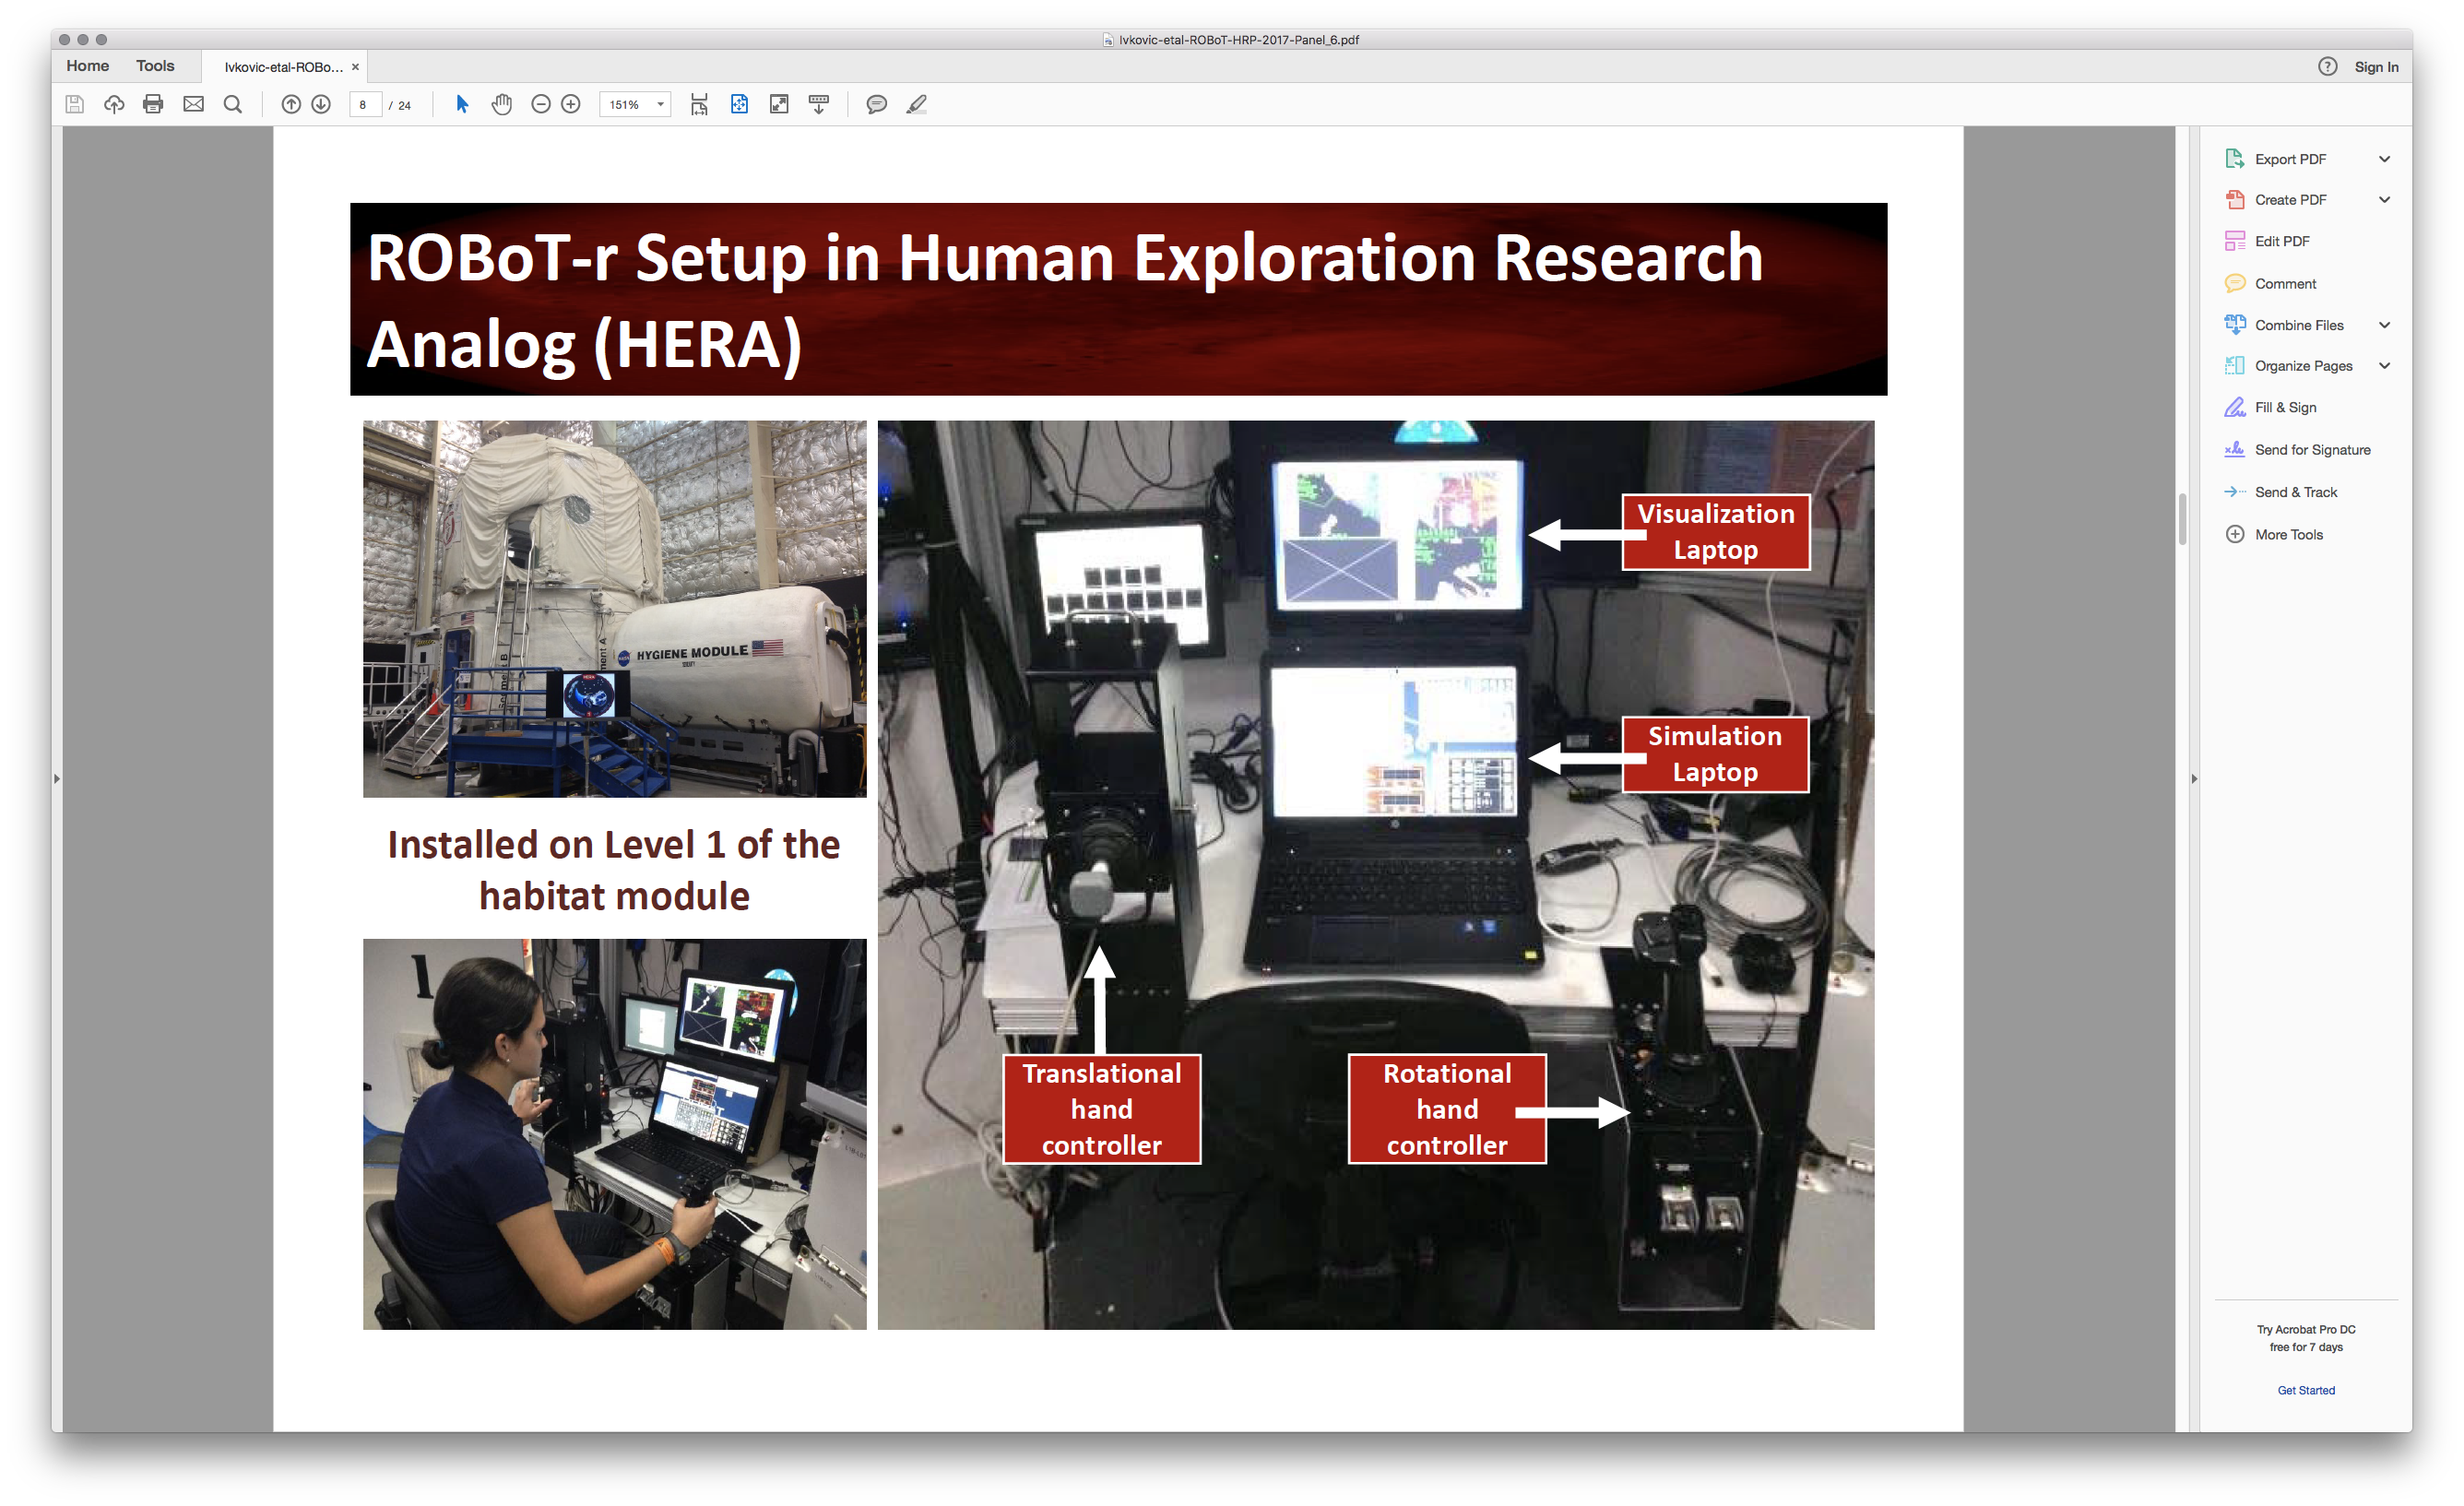
\includegraphics[trim={13cm 5cm 22cm 15.5cm},clip,width=\linewidth]{./../img/Screen Shot 2018-07-26 at 1.43.16 PM.png}
        \caption{The Robotic Onboard Trainer (ROBoT) station set up in the NASA HERA Analog.}
        % \label{}
    \end{center}
\end{figure}

\begin{figure}[tb!]
    \begin{center}
        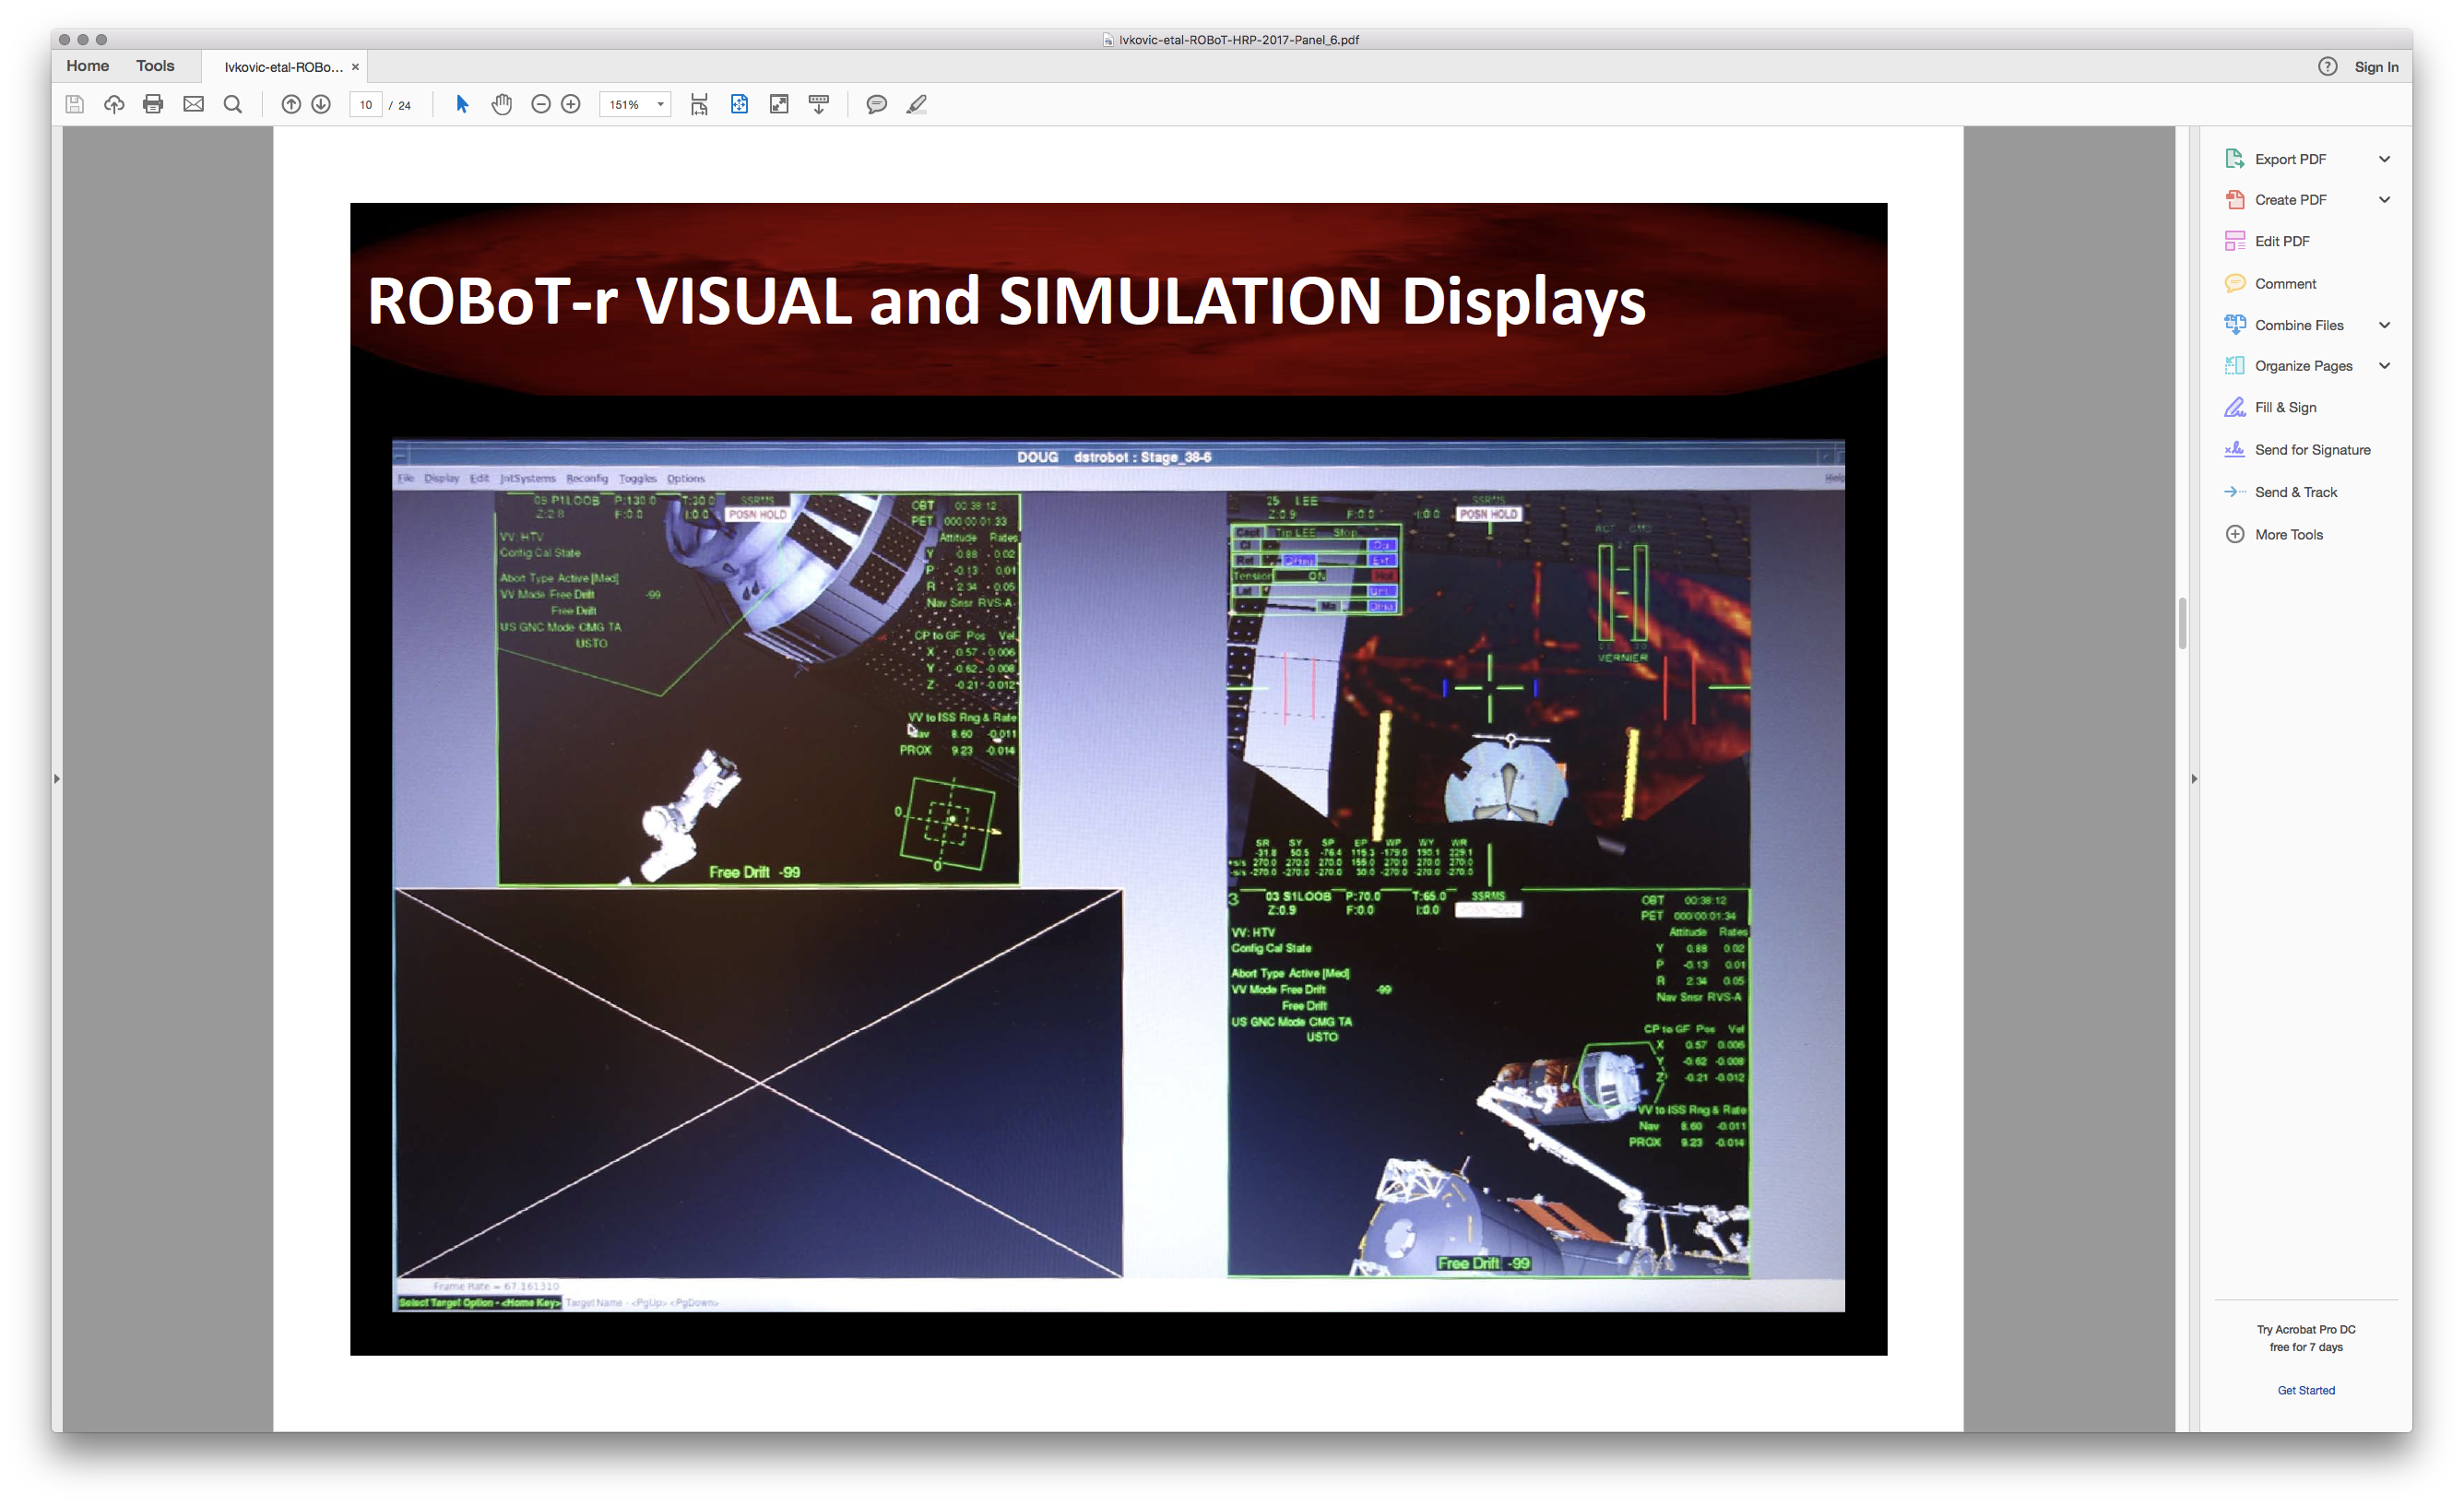
\includegraphics[trim={13cm 5cm 22cm 15.5cm},clip,width=\linewidth]{./../img/Screen Shot 2018-07-26 at 1.43.02 PM.png}
        \caption{ROBoT visualization laptop, showing four camera views.}
        % \label{}
    \end{center}
\end{figure}

\begin{figure}[tb!]
    \begin{center}
        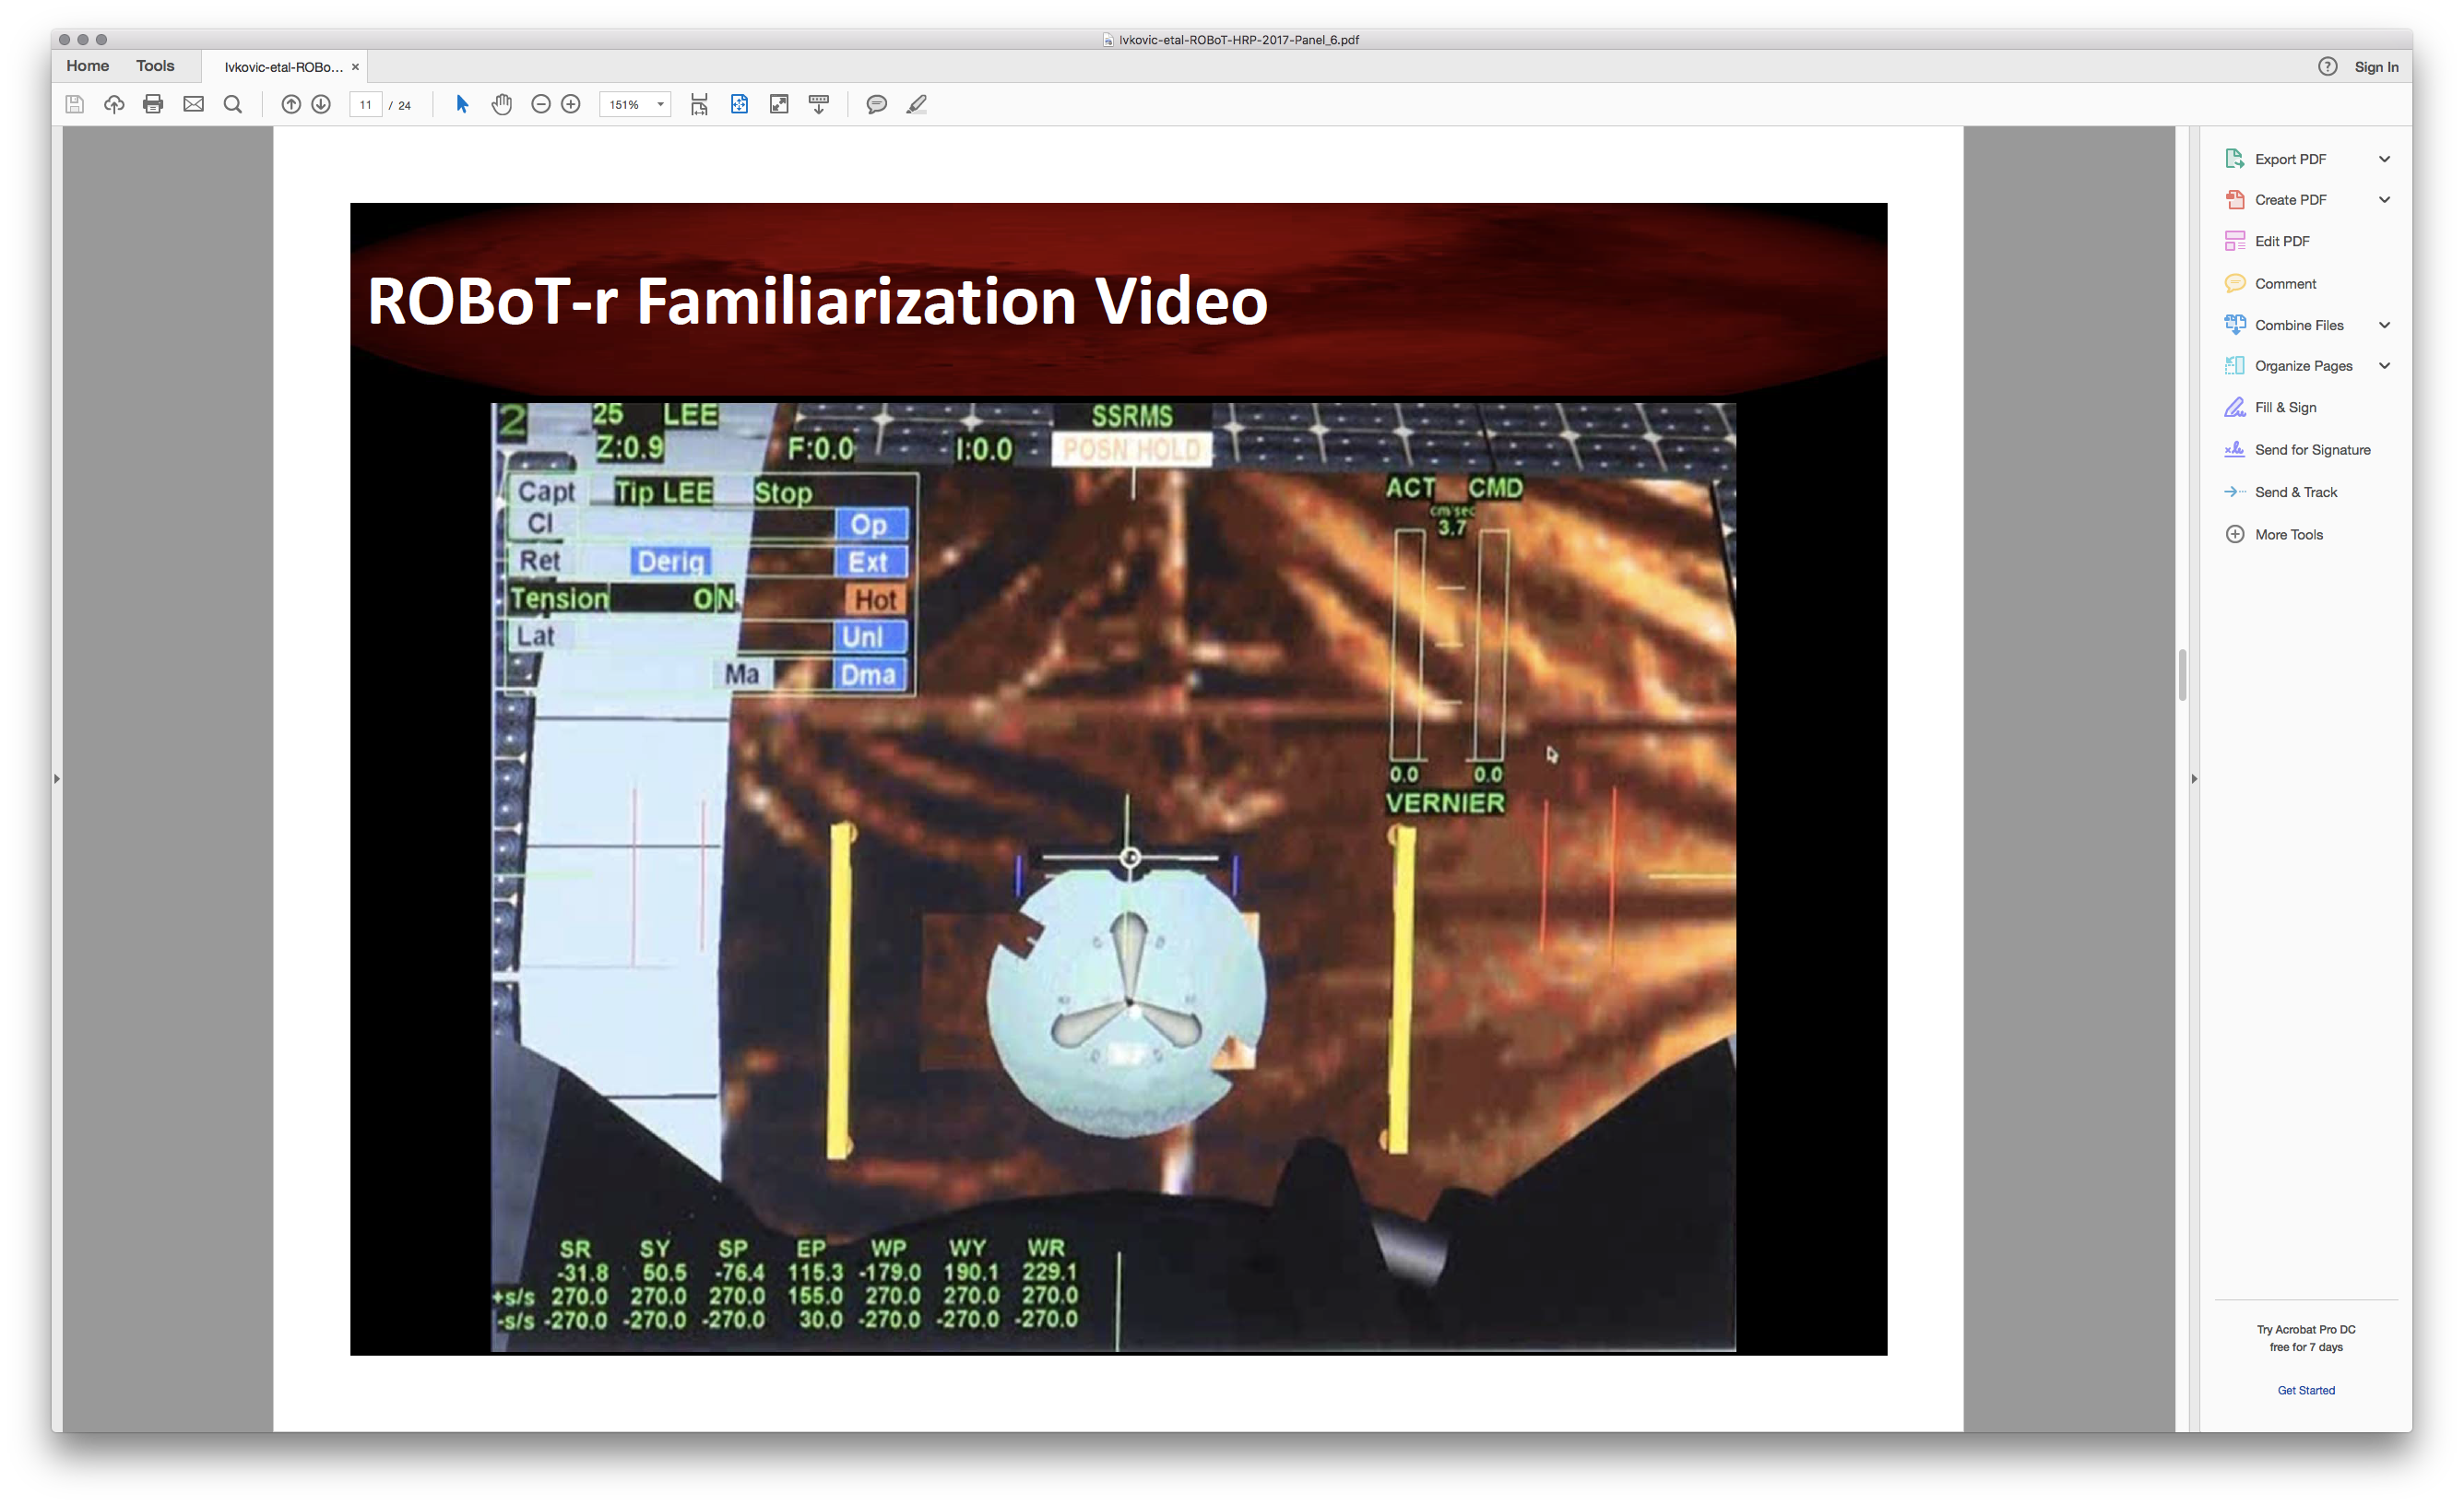
\includegraphics[trim={13cm 5cm 22cm 15.5cm},clip,width=\linewidth]{./../img/Screen Shot 2018-07-26 at 1.43.05 PM.png}
        \caption{The camera attached to the end effector of the robotic arm, showing the grapple fixture.}
        % \label{}
    \end{center}
\end{figure}

% \begin{figure}[tb!]
%     \begin{center}
%         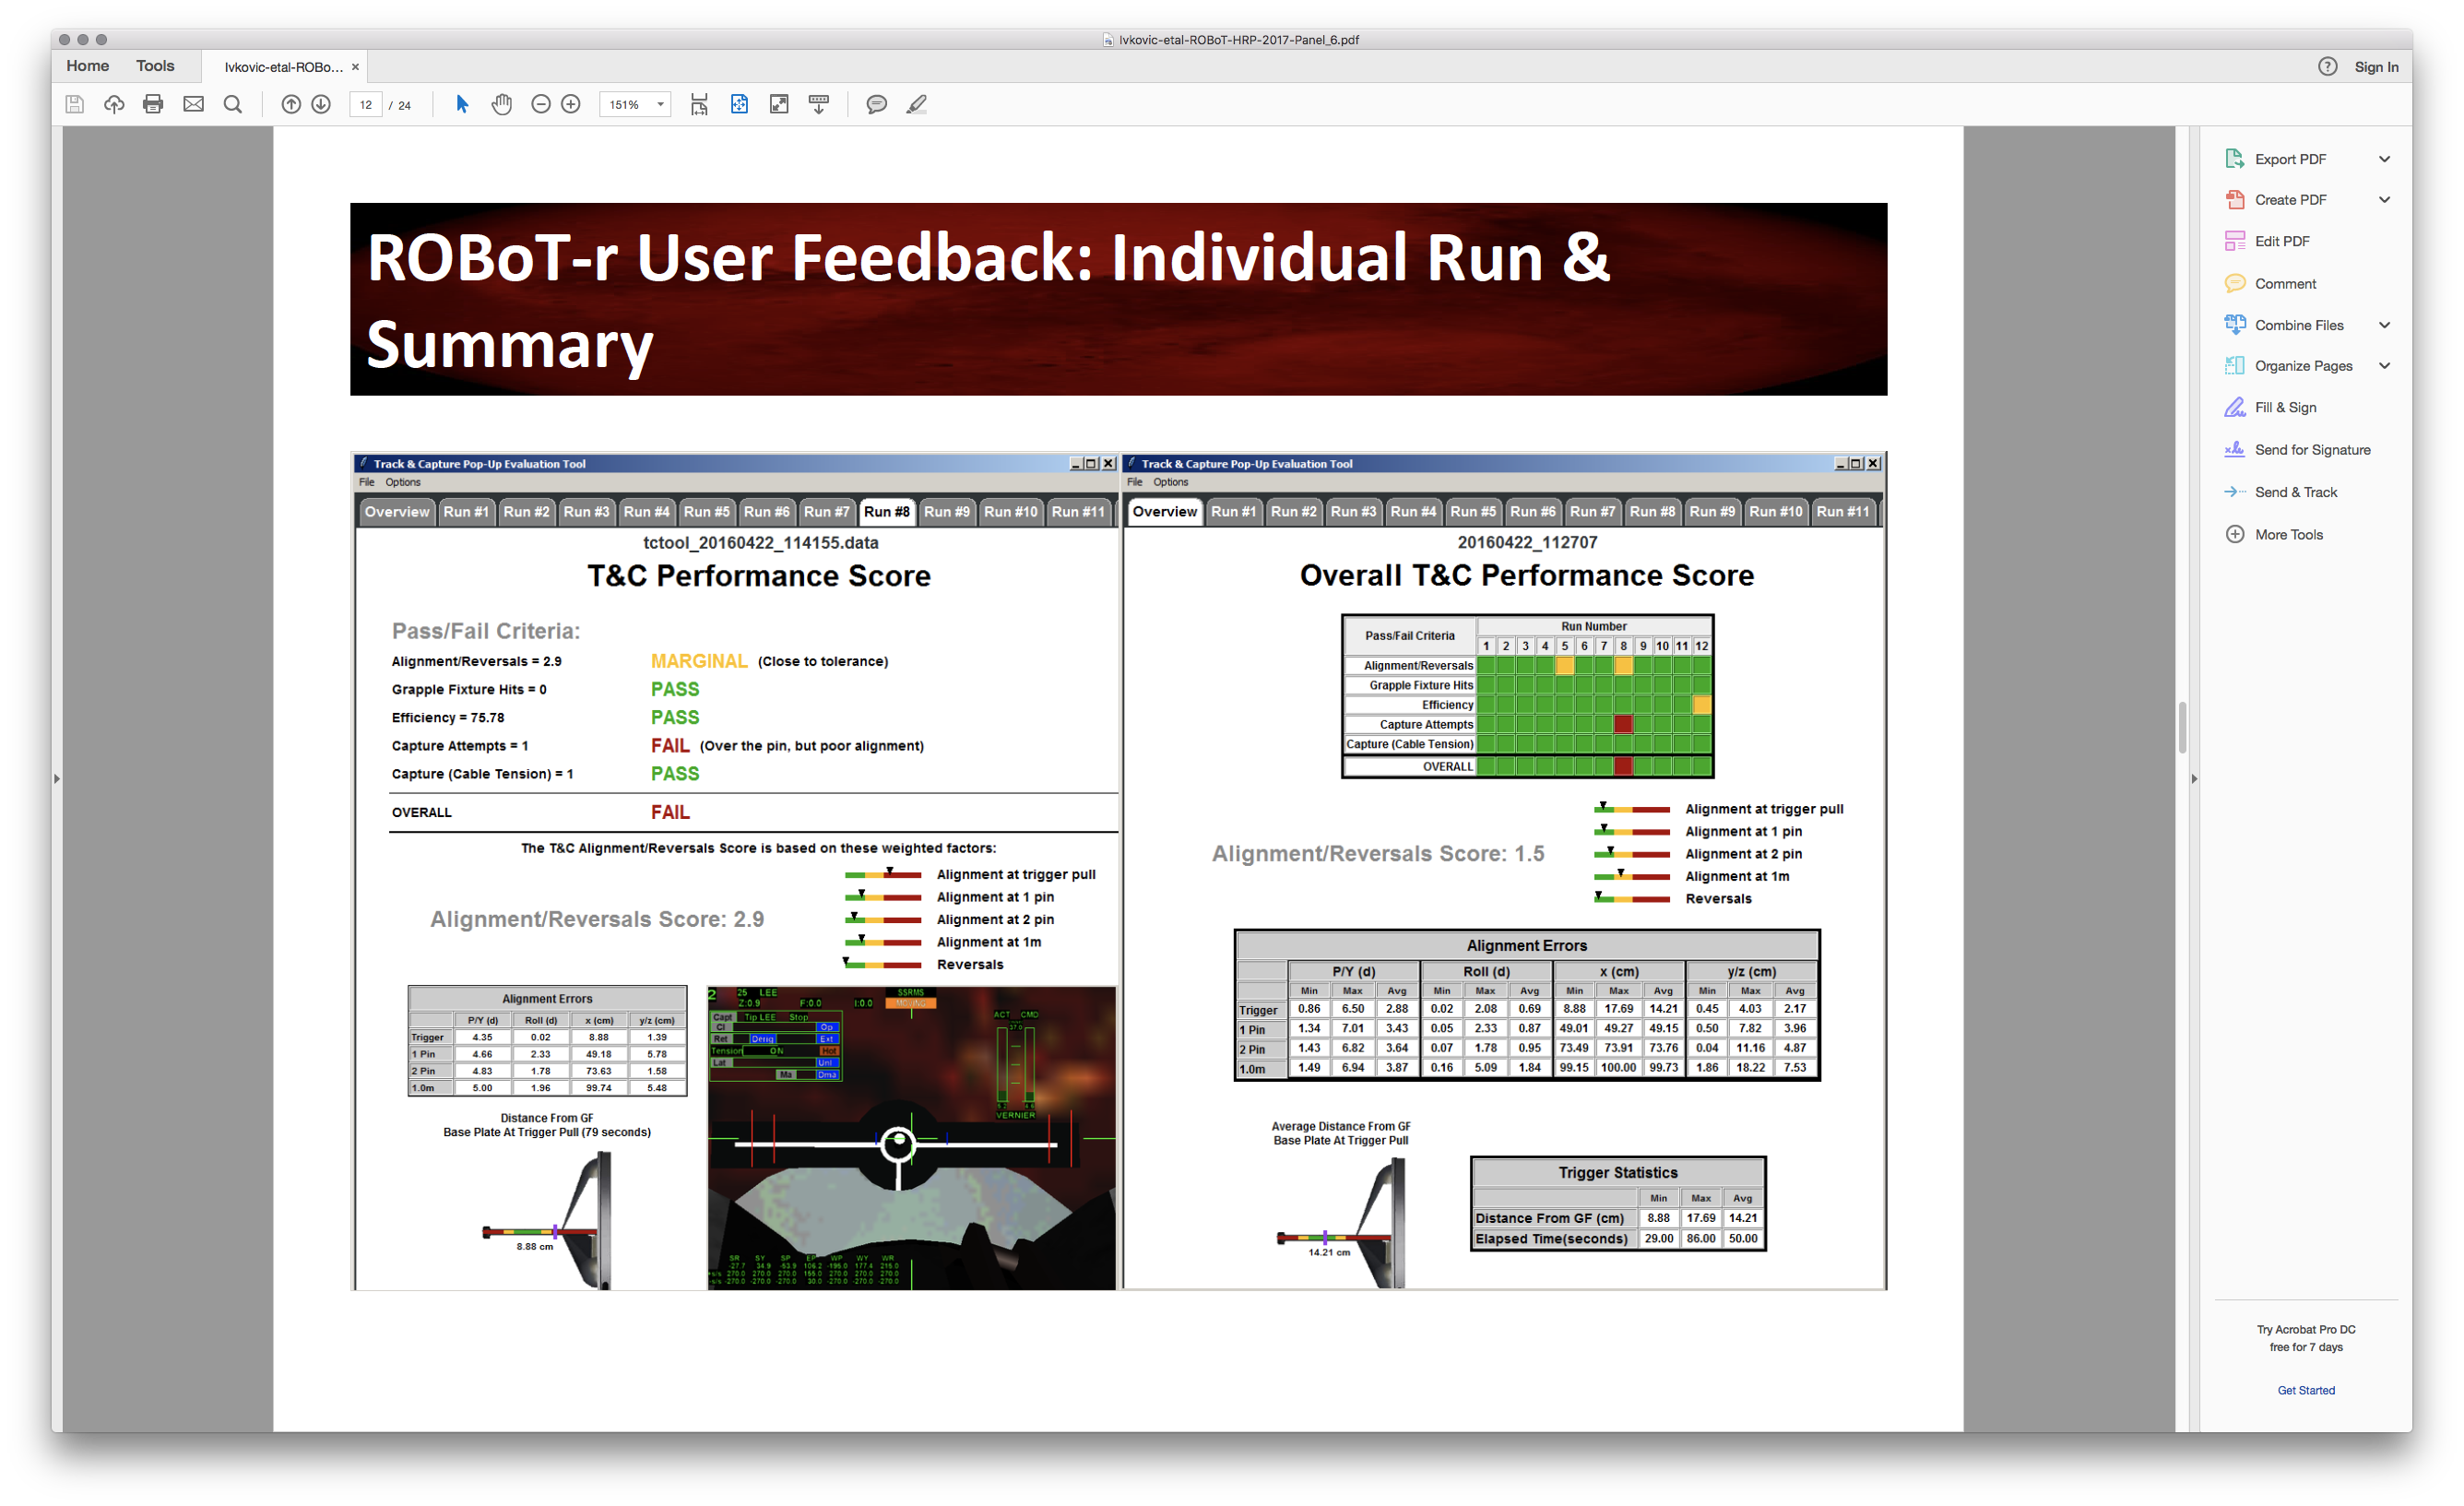
\includegraphics[trim={13cm 5cm 22cm 15.5cm},clip,width=\linewidth]{./../img/Screen Shot 2018-07-26 at 1.43.07 PM.png}
%         \caption{Example performance score report shown to the user after each trial.}
%         % \label{}
%     \end{center}
% \end{figure}

% \begin{figure}[tb!]
%     \begin{center}
%         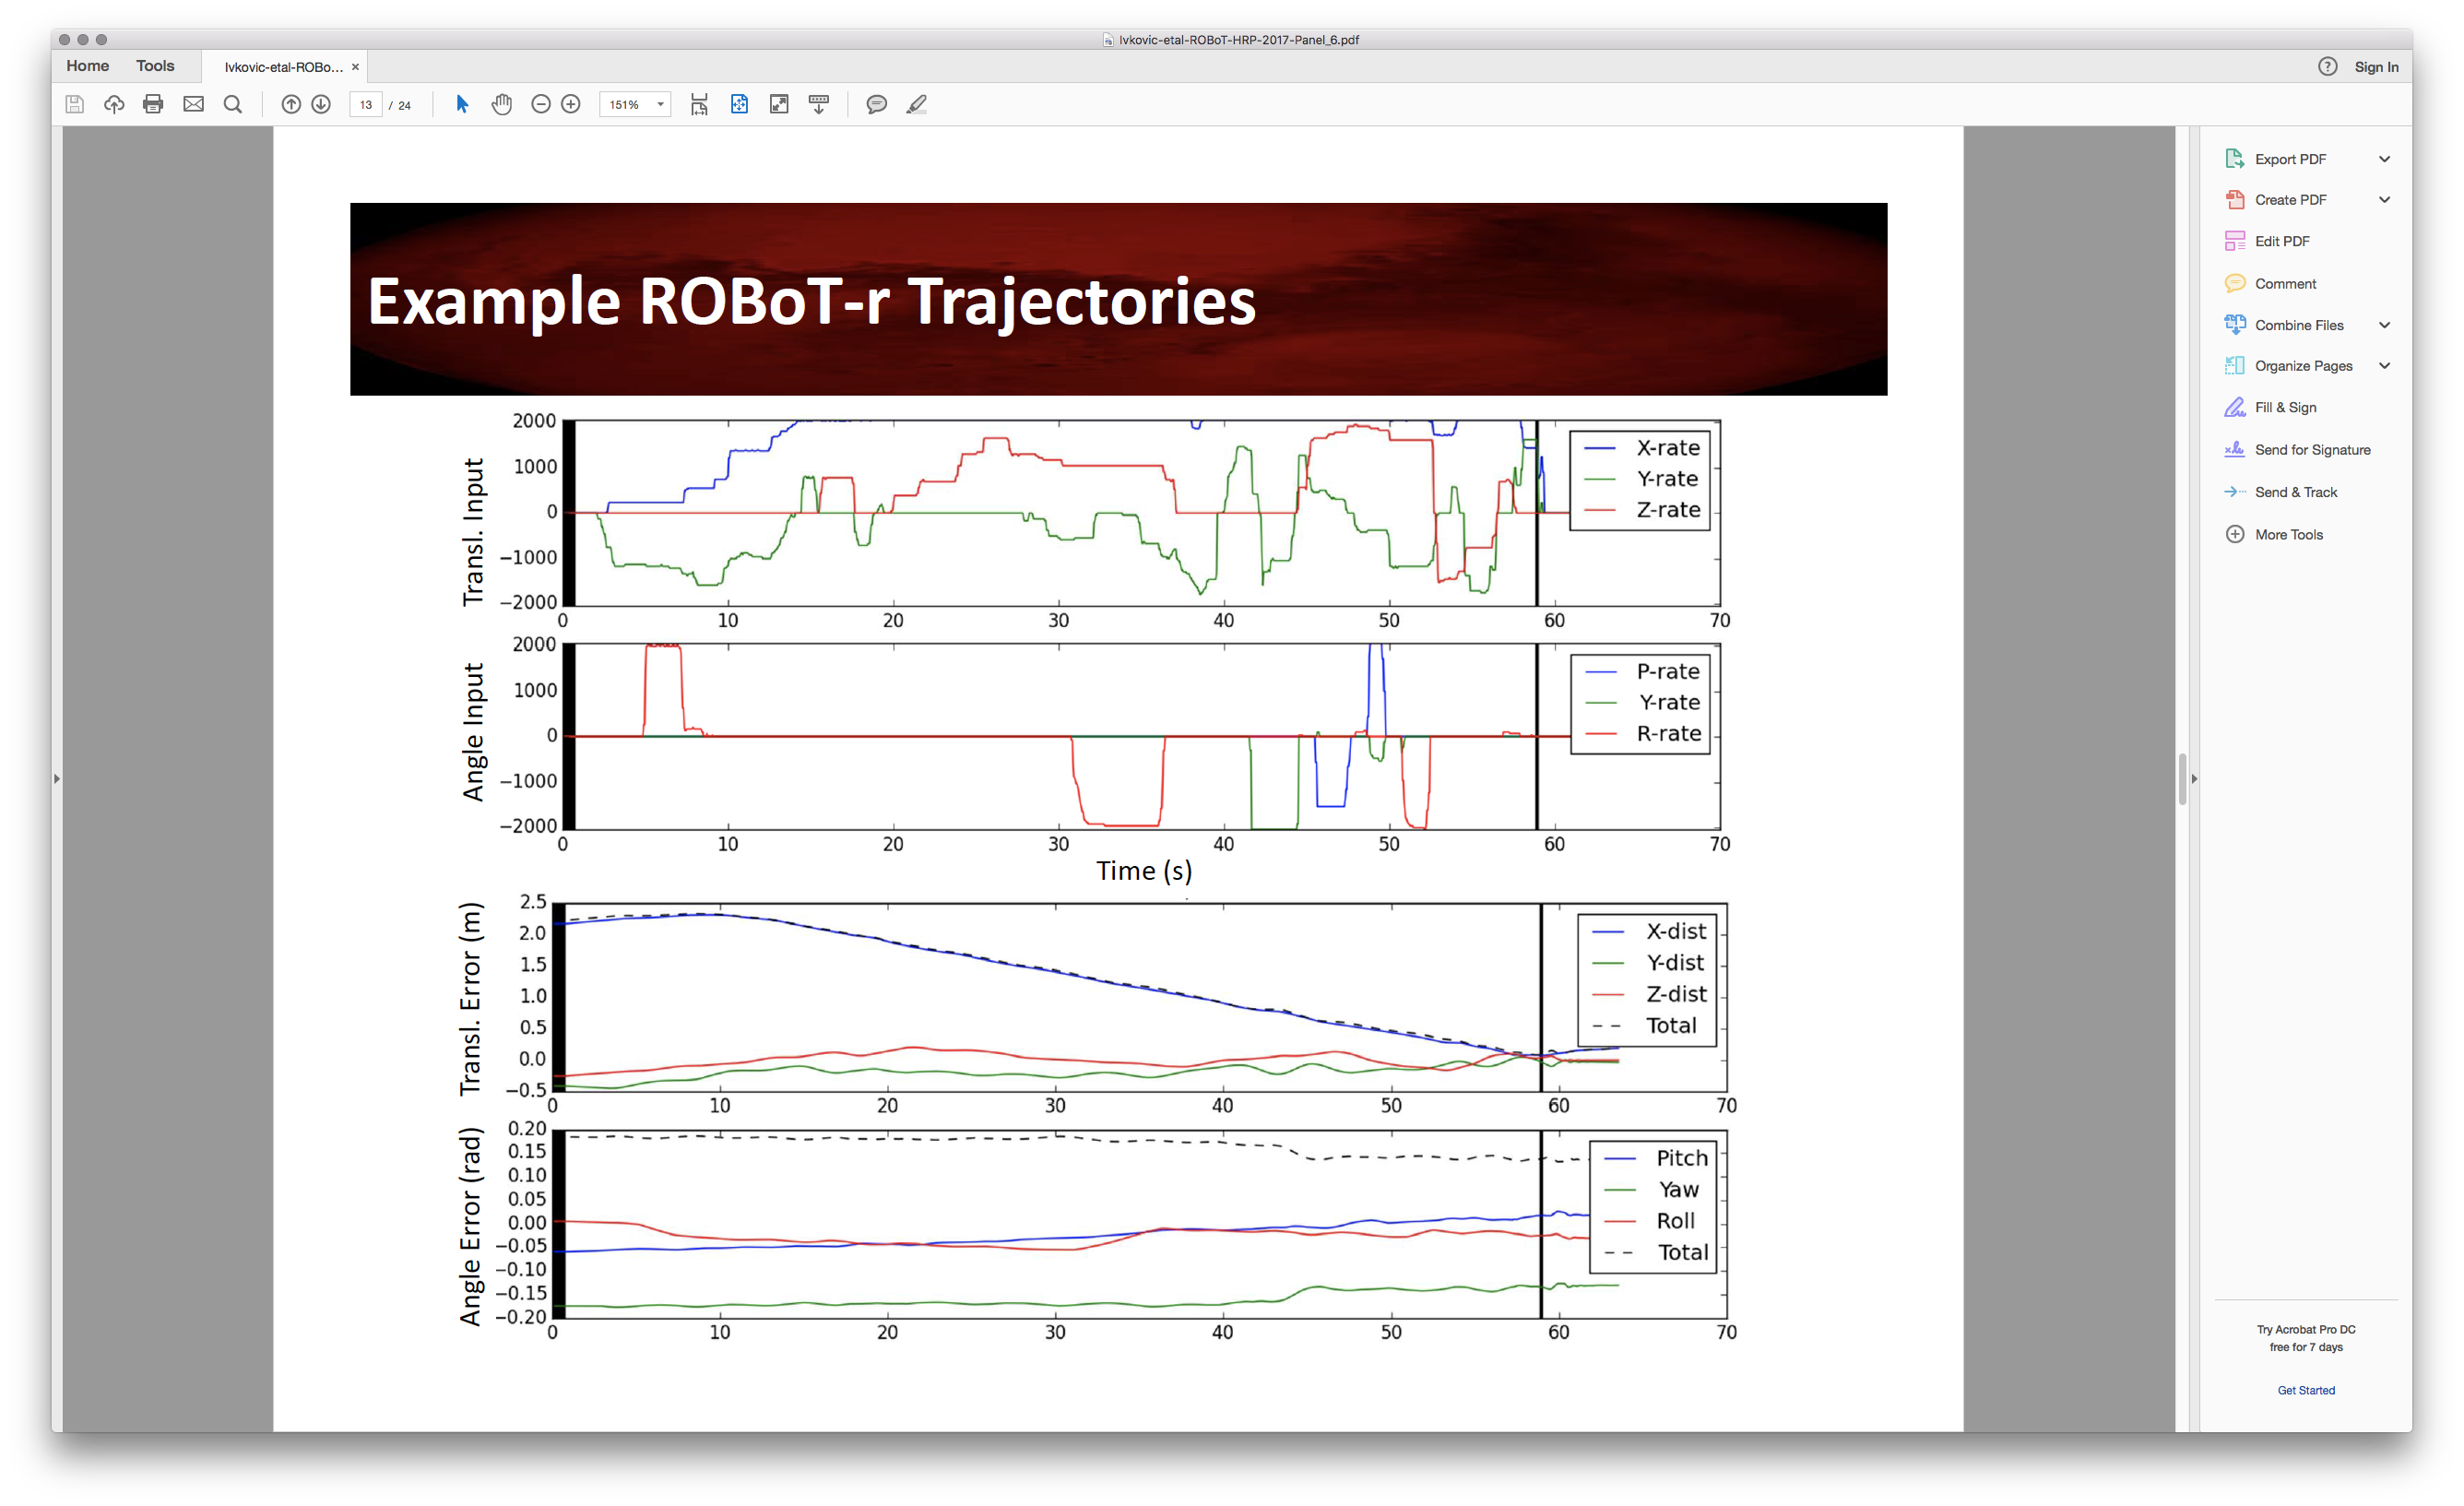
\includegraphics[trim={13cm 5cm 22cm 15.5cm},clip,width=\linewidth]{./../img/Screen Shot 2018-07-26 at 1.43.10 PM.png}
%         \caption{The hand controller inputs and position and angular errors are also logged throughout the trial.}
%         % \label{}
%     \end{center}
% \end{figure}


\subsection{Model Extension}
The Model will extend Professor Hess’ structural model of the human pilot to include the effects of concurrent bandwidth feedback.
The outputs of this model will be compared to the results of Experiment One and Two.

\subsection{Timeline}

\begin{figure}[h!]
    \begin{center}
        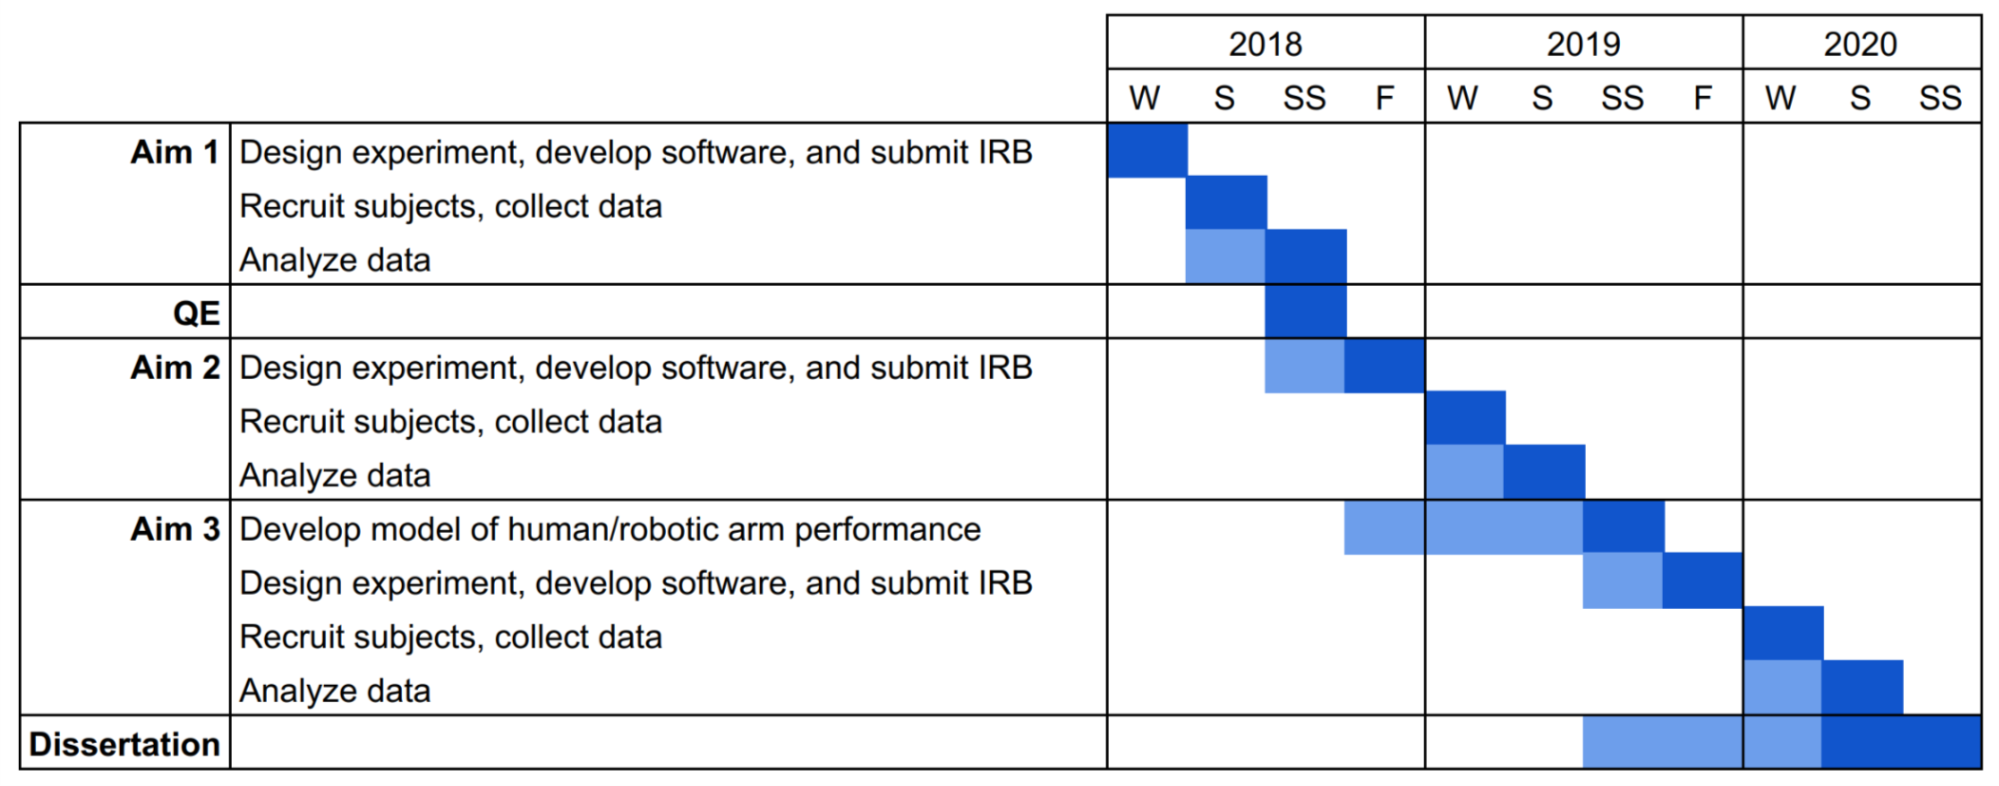
\includegraphics[width=\linewidth]{./../img/image1.png}
        % \caption{}
        % \label{}
    \end{center}
\end{figure}

\end{document}
